\subsection{Desarrollo de la funcionalidades básicas}
\label{sec:desarrollo_funcionalidades_basicas}

En esta sección se va a desarrollar el proceso de implementación de las funcionalidades básicas de la aplicación OTT.
Como ya se indicó en anteriores puntos, las tecnologías utilizadas pra el desarrollo de la aplicación son JavaScript, HTML y CSS.

\subsubsection{Indicaciones previas}
\label{sec:indicaciones_previas}

Esta sección va a describir el comportamiento básico de la aplicación cuando está siendo utilizada en televisiones ya que
es el enfoque principal de la aplicación en estos momentos y es el enfoque que más desafios supuso durante el desarrollo del código.

Trabajar en aplicaciones para televisiones tiene una particularidad y es que hay diseñar la aplicación para ser utilizada
con un mando a distancia. Aunque en algunas televisiones existe la posibilidad de utilizar el "magic remote" que es un mando
a distancia que tiene un puntero que se mueve por la pantalla, la mayoría de las televisiones no tienen esta funcionalidad y
desarrollar la aplicacion únicamente para televisores con esta opción sería un error ya que limita mucho el mercado al que
se puede llegar. Es por eso que la aplicación esta desarrollada desde un punto de vista que permita ser utilizada con un mando
a distancia. Aun así, se ha tenido en cuenta la posibilidad de que la aplicación pueda ser utilizada con un puntero o un ratón
en el caso de los ordenadores ya que, aunque no fue un objetivo para las primeras versiones de la aplicación, uno de los objetivos del 
código es que sea transversal y pueda ser utilizado en cualquier dispositivo. 

\subsubsection{Creación de los componentes de la aplicación}
\label{sec:creacion_componentes_aplicacion}

El primer paso del desarrollo fue la creación de la estructura básica de la aplicación de los primeros componentes que se iban a utilizar y 
sobre los que se ejecutan las funcionalidades básicas de la aplicación. Estos componentes son los menús, los "widgets" y los contenidos.

La creación de estos componentes es una creación en cascada podriamos decir. Cuando se inicia la aplicación, se llama a través de la 
API de la empresa a lo que internamente conocemos como "interfaz". Esta interfaz es un JSON que contiene toda la información principal de la aplicación
y con la que se dan los primeros pasos de creación de la misma. En este JSON tendremos los colores utilizados a lo largo de toda la aplicacion (colores de fondo,
de los botones, de los textos, etc), las fuentes de texto, textos legales, imagenes (logos, splash, etc) y demás información que se utilizará para la personalización
para cada cliente de la aplicación. Dentro de esta información también se encuentra la información de los distintos menús que va a tener la aplicación. 

Para la creación de cada uno de estos menús existen dos opciones: que tengan una pantalla asignada o que sean menús con un comportamiento predefinido. Dentro de 
de los menús con comportamientos predefinidos encontramos los menús de configuración o perfil, de búsqueda y de catálogo. Estos casos tienen un comportamiento
específico y no necesitan la información sobre la pantalla que deben mostrar. 

\begin{itemize}
    \item \textbf{Configuración:} Este  menú alojará las distintas opciones de configuración que tenga cada aplicación. No siempre son las mismas, pero en función 
    de las características de la aplicación se mostrarán unas u otras. Si la aplicación para determinado cliente debe soportar multilenugaje, en este menú se podrá
    cambiar el idioma de la aplicación. Si la aplicación tiene usuarios registrados, se mostrará la información del usuario y se podrá cerrar sesión. Una funcionalidad
    que aparece en todas las aplicaciones es la de mostrar los términos y condiciones de la aplicación. Para otras funcionalidades hay que acordar con el cliente 
    pertinente los requisitos y se añadiria para su aplicación la funcionabilidad necesaria. 
    \item \textbf{Búsqueda:} Este menú alojará la funcionalidad de búsqueda de la aplicación. En este menú se podrá filtar todos los contenidos de la aplicación
    por el nombre del contenido.
    \item \textbf{Catálogo:} También conocido como "A la carta" permite mostrar en la misma página todos los contenidos disponibles para ver en la aplicación.
\end{itemize}

En el caso de los menús que tienen una pantalla asignada, esta pantalla contiene la lista de los "widgets" que se deben mostrar en ella. Estos widgets son contenedores
de elementos y cada uno en función de su tipo tendrá un diseño y unas funcionalidades asignadas. A su vez, para cada uno de estos widgets existirá una lista de los contenidos
junto con la información de cada uno de ellos. 

Por lo tanto, la creación de las pantallas principales se realiza de la siguiente manera:

\begin{itemize}
    \item Se consigue la información del menú a través de la API.
    \item Se analiza para saber si es un menú predefinido o si tiene una pantalla asignada. \begin{itemize}
        \item Si es un menú predefinido, se crea la pantalla según el comportamiento predefinido.
        \item Si tiene una pantalla asignada, se consigue la información de la pantalla. \begin{itemize}
            \item Se crea el elemento del DOM que contendrá la pantalla.
            \item A partir de la lista de widgets, se crea un elemento del DOM para cada uno de ellos.
            \item Se consigue la información de los contenidos de cada widget.
            \item Se crea cada uno de los contenidos con las características correspondientes en función del tipo del widget que los contiene.
            \item Se añade cada contenido al widget correspondiente según el orden correspondiente.
            \item Se añade el widget al elemento del DOM que contiene la pantalla.
        \end{itemize}
    \end{itemize}
\end{itemize}

A lo largo de la creación de cada elemento html se le irá asignando según el tipo de elemento y widget correspondiente una serie de clases que permitirán
darle el estilo gracias a las hojas de estilo CSS.

El tipo de widget también determina el comportamiento de los contenidos que contiene. Por ejemplo, si el widget es de tipo "featured" con el campo "slider" activado, 
los contenidos destacados se mostrarán en un carrusel. Si el widget es de tipo "mosaico" los contenidos se mostrarán en una cuadrícula y el movimiento en 
lugar de ser una lista que se mueve horizontalmente, será una cuadrícula que se mueve en ambas direcciones.

\subsubsection{Movimiento por la aplicación}
\label{sec:movimiento_aplicacion}

Una vez creados los elementos de la aplicación, el siguiente paso es poder movernos por ella. Para ello, se ha creado una serie de funciones que permiten
moverse por los distintos elementos de la aplicación. Para este punto se ha tenido en cuenta que la aplicación pueda ser utilizada con un mando a distancia
y por lo tanto, ese movimiento debe de estar desarrollado y controlado por el código. 

Cuando la aplicación se utiliza en televisión hay que tener en cuenta que se debe tener un foco en un elemento en todo momento. Este foco es el que indica
en qué elemento de la aplicación se encuentra el usuario y es el que permite moverse por la aplicación. Para esta aplicación, en las pantallas principales
se ha utilizado un foco fijo, es decir, por norma general el foco se encuentra siempre en la misma posición y son los elementos los que se mueven en función
de la dirección en la que se mueva el usuario hacia ese foco. 

El movimiento por los widgets se realiza de la siguiente manera:
\begin{itemize}
    \item \textbf{Movimiento horizontal:} El movimiento horizontal se realiza con las teclas de dirección izquierda y derecha. Si estamos en un widget, el movimiento
    se realizará en los contenidos del widget. Cada vez que se pulsa una tecla de dirección, el widget se mueve horizontalmente en función de la dirección en la que se 
    haya pulsado colocando el elemento seleccionado en la posición del foco.
    \item \textbf{Movimiento vertical:} El movimiento vertical se realiza con las teclas de dirección arriba y abajo. Si estamos en una pantalla y todavía quedan widgets
    por mostrar hacia la dirección en la que se ha pulsado, se desplazará la pantalla hacia arriba o hacia abajo en función de la dirección en la que se haya pulsado 
    hasta colocar el elemento seleccionado en la posición del foco.
    \item \textbf{Movimiento en carrusel:} En el caso de que el widget sea de tipo "featured" y tenga el campo "slider" activado, el movimiento se realizará en el carrusel
    de los contenidos destacados. En este caso, el movimiento horizontal cambiará la imagen y la información mostrada en el carrusel.
    \item \textbf{Movimiento en mosaico:} En el caso de que el widget sea de tipo "mosaico", el movimiento se realizará en la cuadrícula de los contenidos. En este caso
    los contenidos aparecen ordenados por filas de izquierda a derecha y de arriba a abajo. el movimiento vertical desplazará la pantalla hacia arriba o hacia abajo
    en función de la dirección en la que se haya pulsado y el movimiento horizontal en este caso en concreto sí que moverá el foco hacia el elemento seleccionado.
\end{itemize}

Por otro lado el movimiento por el menú lateral es más simple. Para acceder al menú lateral hay varias opciones: se puede acceder pulsando el boton "return" siempre y 
cuando estemos en una pantalla principal o se puede acceder pulsando la tecla "izquierda" siempre y cuando no queden más elementos a la izquierda. Una vez seleccionado
el menú este se despliega ocupando más sitio y muestra no solo los iconos si no también los nombres de los menús. Para moverse por el menú se utilizarán las teclas de 
arriba y abajo y el foco hará que el elemento seleccionado destaque en tamaño. 

\begin{figure}[H]
    \centering
    \begin{subfigure}[c]{0.1\textwidth} 
        
\includegraphics[width=\textwidth]{imaxes/OTT/menu_lateral_cerrado.png}
        \subcaption{Menú lateral colapsado}
        \label{fig:Widget_banner}
    \end{subfigure}
    \hspace{0.05\textwidth}
    \begin{subfigure}[c]{0.1\textwidth}
        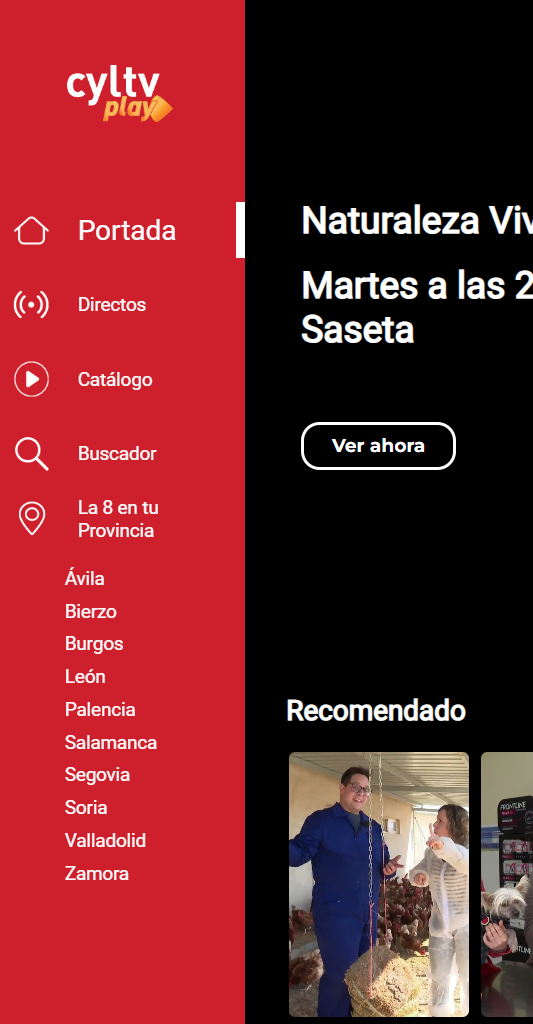
\includegraphics[width=\textwidth]{imaxes/OTT/menu_lateral_abierto.png}
        \subcaption{Menú lateral abierto}
        \label{fig:Widget_mosaico}
    \end{subfigure}
    \caption{Menú lateral}
\end{figure}

    

\subsubsection{Selección de un componente}
\label{sec:seleccion_componente}

Una vez que se ha movido el foco al elemento deseado, el siguiente paso es seleccionar ese elemento. Para ello, cada componenete tiene asociado un evento de selección
que se activa cuando se pulsa el botón de selección del mando a distancia. Este evento de selección es el que permite realizar la acción correspondiente al elemento
seleccionado. 

Estos eventos pueden ser creación de una nueva pantalla (en el caso de seleccionar una opción del menú lateral) o creación de una pantalla de detalle
(en el caso de seleccionar un contenido). En el caso de crear una nueva pantalla, se seguirá el mismo proceso que se ha seguido para la creación de la pantalla principal
y se mostrará la nueva pantalla en la aplicación, almacenando la pantalla anterior en una pila de pantallas. En el caso de seleccionar un contenido, se creará una pantalla
de detalle con la información del contenido seleccionado.

\subsubsection{Creación de la pantalla de detalle}
\label{sec:creacion_pantalla_detalle}

La pantalla de detalle es una pantalla que muestra la información detallada de un contenido. Esta pantalla se crea en función de la información que se 
recibe tras realizar una llamada a la API con el identificador del contenido seleccionado.

Existen dos tipos de pantallas de detalle en función del tipo del contenido: los contenedores y los contenidos. Los contenedores son aquellos contenidos que
contienen otros contenidos. Por ejemplo, una serie es un contenedor que contiene los capítulos de la serie. Los contenidos son elementos finales, como una película,
un capitulo, una partido, etc. Estos no tienen hijos asociados.

La pantalla de detalle de un contenedor está compuesta por una ficha con la información del elemento , una lista de los contenidos que contiene y una lista de los
contenedores relacionados. Para moverse por lo contenidos hijos haremos uso del movimiento vertical de igual forma que en la pantalla principal y una vez estemos 
en los contenidos relacionados el funcionamiento es el mismo que el de los widgets de la pantalla principal con el movimiento horizontal.

\begin{figure}[H]
    \begin{subfigure}[c]{0.5\textwidth}
        \includegraphics[width=\textwidth]{imaxes/OTT/pantalla_detalle_contenedor1.png}
        \subcaption{Pantalla de detalle de un contenedor}
        \label{fig:Widget_banner}
    \end{subfigure}
    \hspace{0.1\textwidth}
    \begin{subfigure}[c]{0.5\textwidth}
        \includegraphics[width=\textwidth]{imaxes/OTT/pantalla_detalle_contenedor2.png}
        \subcaption{Pantalla de detalle de un contenedor}
        \label{fig:Widget_mosaico}
    \end{subfigure}
    \caption{Pantalla de detalle de un contenedor}
\end{figure}

Por otro lado, la pantalla de detalle de contenido está compuesta por una ficha con la información del contenido, donde se incluye el titulo, contenedor padre (si lo
tiene , en el caso de un capitulo de una serie, la serie a la que pertenece), una descripción corta, un botón que permite mostrar un popup con todo la información al 
completo, los iconos de rating y edad, un botón de reproducción y en caso de permitir la funcionalidad, un botón de añadir a favoritos. También tiene una lista de
contenidos relacionados.

\begin{figure}[H]
    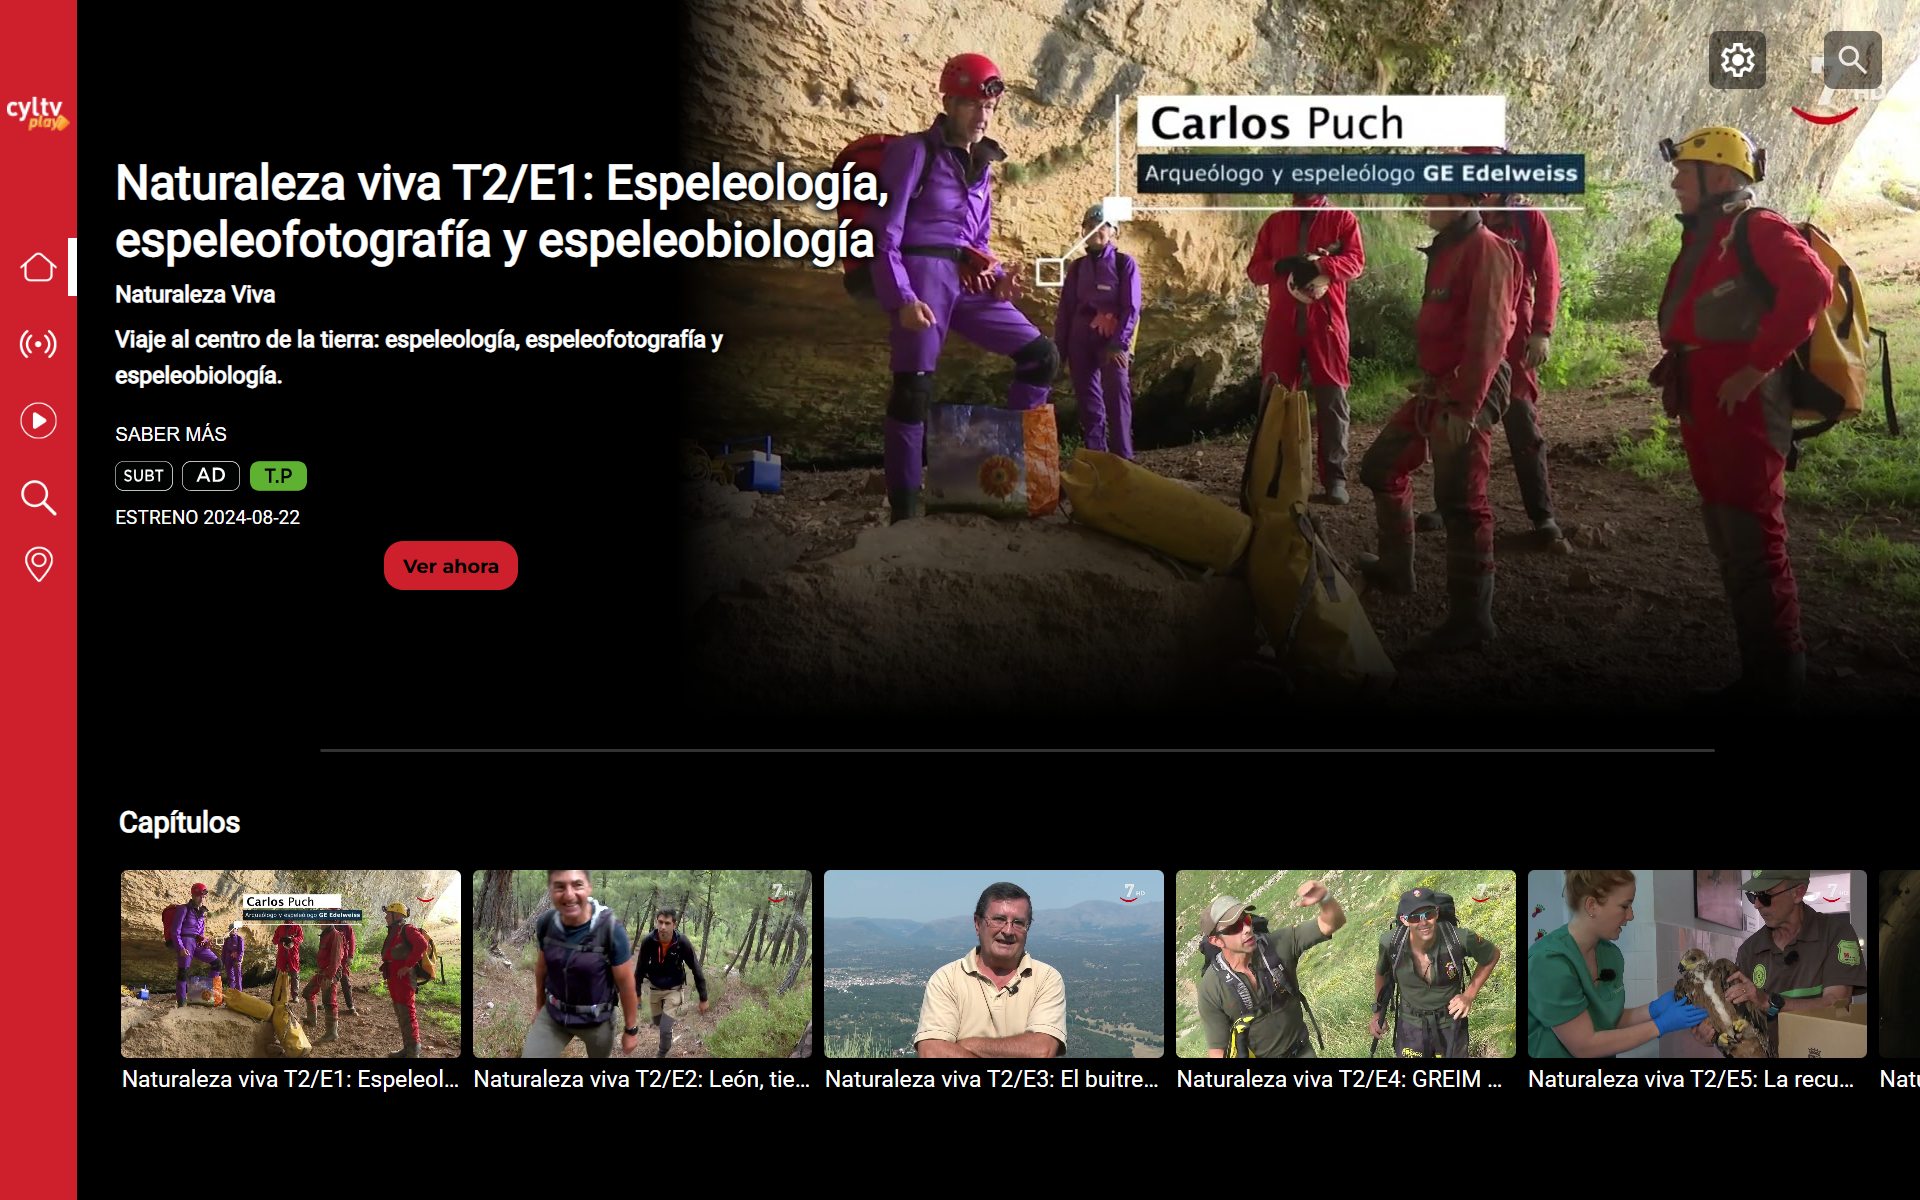
\includegraphics[width=0.4\textwidth]{imaxes/OTT/Pantalla_detalle_contenido.png}
    \caption{Pantalla de detalle}
\end{figure}

\subsubsection{Reproducción de un contenido}
\label{sec:reproduccion_contenido}

La reproducción de un contenido es una de las funcionalidades más importantes de la aplicación. Para acceder a ella hay dos opciones: a través de la pantalla de detalle
de contenido explicada en el punto anterior, o si un contenido tiene el trigger de reproducción activado, se podrá acceder a la reproducción directamente desde la pantalla
principal. Al seleccionar el botón de reproducción, la aplicación obtiene la información del contenido. En esta información se comprueba si el contenido 
necesita autentificación para ser reproducido y en caso afirmativo (el usuario ya deberia estar logueado) se comprueba si el usuario tiene permisos para ver el contenido.
Es una comprobación de seguridad ya que en caso de no tener acceso al contenido el botón de reproducción aparece como deshabilitado. En caso de tener acceso, el 
se realizan varias comprobaciones:

\paragraph{Origen del contenido:} Lo primero es comprobar de donde proviene el contenido. Aqui hay dos opciones: o esta alojado en la base de datos de la empresa o 
en la del cliente. Si esta en la del cliente la url del video estará ya en la información del contenido. En caso de estar en la base de datos de la empresa, hay que 
realizar una serie de comprobaciones para obtener la url del video. Estas comprobaciones son en base a si el contenido es gratuito o de pago ya que si es
gratuito la url se podra montar directamente con la información que se tiene, pero si es de pago hay que realizar una serie de comprobaciones para obtener la información.

\paragraph{Reproductor:} No todos los dispositivos pueden usar el mismo reproductor. Los ordenadores son más permisivos con este detalle, pero las televisiones no. En 
el caso de los ordenadores existe la opción incluso de que la API nos devuelva un player ya construido para utilizar directamente en la aplicación. Este caso no se utiliza
por el momento. Lo hace el código es detectar en que SO y con que contenido se esta trabajando. Aquí tenemos por el momento dos reproductores (VideoJs y ShakaPlayer) y dos 
tipos de video (VoD y Lives o Youtube). Para cada caso se monta el reproductor de una manera especifica. 


Una vez el video se está reproducciendo, el usuario dispone de las funcionalidades básicas para controlar la reproducción: pause, play, adelantar, retroceder y salir. 
En caso de permitir la funcionalidad y tener usuarios registrados la aplicación guarda el instante en el que se detuvo la reproducción para que el usuario pueda
continuar viendo el contenido en el mismo punto en el que lo dejó.

\subsubsection{Añadir a favoritos}
\label{sec:anadir_favoritos}

En caso de permitir usuarios registrados, la aplicación permite añadir a favoritos los contenidos. Para ello, en la pantalla de detalle de contenido se muestra un 
botón en forma de corazón que permite añadir el contenido a favoritos. En caso de que el contenido ya esté añadido a favoritos, el botón aparecerá en color rojo y pulsando
sobre él se eliminará de la lista de favoritos.

\subsubsection{Búsqueda de contenidos}
\label{sec:busqueda_contenidos}

La búsqueda de contenidos es una funcionalidad básica de la aplicación. Para acceder a ella se puede hacer de dos formas: a través del menú lateral o una opción 
situada en la parte superior derecha de todas las pantallas. Al abrir el menú de búsqueda, se muestra un campo de texto en el que se puede introducir el nombre del
contenido que se desea buscar. Una vez escrito el nombre completo o parcial del contenido y hacer click en el botón de búsqueda, la aplicación realiza una llamada a la
API con el nombre del contenido y obtiene una lista de los contenidos que coinciden con el nombre introducido. Esta lista se muestra en una pantalla de resultados de
búsqueda en forma de mosaico. 


\subsubsection{Obtención de la información de un directo}
\label{sec:obtencion_informacion_directo}

La obtención de la información de un directo es una funcionalidad que permite obtener la información de un directo en tiempo real. Para ello, la aplicación realiza una
llamada a la API con el identificador del directo y obtiene la información del directo en tiempo real a través de un epg. Este epg es un JSON que contiene la información
de los contenidos que se van a emitir en un periodo de tiempo determinado. La aplicación analiza este Json y obtiene la información del directo en tiempo real. De esta 
información se obtiene el titulo que se mostrará en el contenido correspondiente, y el progreso, que se calcula a partir de los tiempos de inicio y fin del contenido marcados
en el Json, y se muestra en la barra de progreso del contenido.

